\documentclass[10pt,twocolumn,letterpaper]{article}

\usepackage{cvpr}
\usepackage{times}
\usepackage{epsfig}
\usepackage{graphicx}
\usepackage{amsmath}
\usepackage{amssymb}
\usepackage{booktabs}

% Include other packages here, before hyperref.

% If you comment hyperref and then uncomment it, you should delete
% egpaper.aux before re-running latex.  (Or just hit 'q' on the first latex
% run, let it finish, and you should be clear).
\usepackage[breaklinks=true,bookmarks=false]{hyperref}

\cvprfinalcopy % *** Uncomment this line for the final submission

\def\cvprPaperID{****} % *** Enter the CVPR Paper ID here
\def\httilde{\mbox{\tt\raisebox{-.5ex}{\symbol{126}}}}

% Pages are numbered in submission mode, and unnumbered in camera-readyhttps://www.overleaf.com/project/6437277b83be5faecea25de2
%\ifcvprfinal\pagestyle{empty}\fi
\setcounter{page}{1}
\begin{document}
%%%%%%%%% TITLE
\title{Fairness Aware Multi-Class Image Classification }
\author{Yufeng Yang, Benson Chi, Fan Qiao\\
Department of Computer Science, Rice University\\
{\tt\small yy94@rice.edu; bc62@rice.edu; fq3@rice.edu}
% For a paper whose authors are all at the same institution,
% omit the following lines up until the closing ``}''.
% Additional authors and addresses can be added with ``\and'',
% just like the second author.
% To save space, use either the email address or home page, not both
}

\maketitle
%\thispagestyle{empty}

%%%%%%%%% ABSTRACT
\begin{abstract}
   Imbalanced dataset is common in real world. One concern using imbalanced dataset for training a neural network is the possible high misclassification rate, which might cause unfairness issues for minority case. In this project, we explore different aspects such as changing loss functions and optimization strategies, modifying neural network architectures, utilizing transfer learning and multi-mode learning to improve the overall classification accuracy over an imbalanced dataset. Results indicate that utilizing vision transformer, initialized knowledge learned from ImageNet1k and image to text technique can significantly improve the accuracy. Especially, by utilizing pre-trained ViT-GPT2 with FlanT5 can achieve 100$\%$ validation accuracy. Explanations of the experiments' design and results are given in the body paragraph. Hopefully, this project will inspire future work on Fair AI with more complicated dataset and tasks. The implementation code can be found  \href{https://drive.google.com/file/d/1mABSGeTZZYIpDUBeLx3tYdxOh_GtiS4D/view?usp=sharing}{here}.
\end{abstract}




%%%%%%%%% BODY TEXT
%%%% Yufeng Yang: I have already modified this part.
\section{Introduction}
Deep Learning has made great success in many application areas such as image classification, image segmentation and multi-mode learning. However, to achieve a good performance under various environments, the high quality of dataset is required. This is not common in reality. There exists extreme cases such as X-ray images for a rare disease, images from rare animals, which are very hard to obtain. The imbalanced data may have significant effect on overall image classification accuracy due to the lack of training images from some specific classes. In this work, we will investigate several different network structures and learning paradigms, which are aimed to improve the overall classification accuracy over a imbalanced data set under limited computing resources.\\



\section{Sampling Imbalanced Dataset}
In this work, we mainly use the dataset introduced from \cite{inproceedings}. The original data sample is equal for each class. To further sample the imbalanced dataset, an uniformly random number $p_i$ from $\left [ 0.4, 0.8 \right ]$ is used to simulate the imbalance distribution over each label $i$. Then,a Bernoulli random variable with probability $p_i$ is used to randomly select samples from a class. The generated dataset can be divided into 6 categories as the table \ref{dataset} shows. Clearly the forest class can be viewed as "minority" group in our dataset.
\begin{figure}
    \centering
    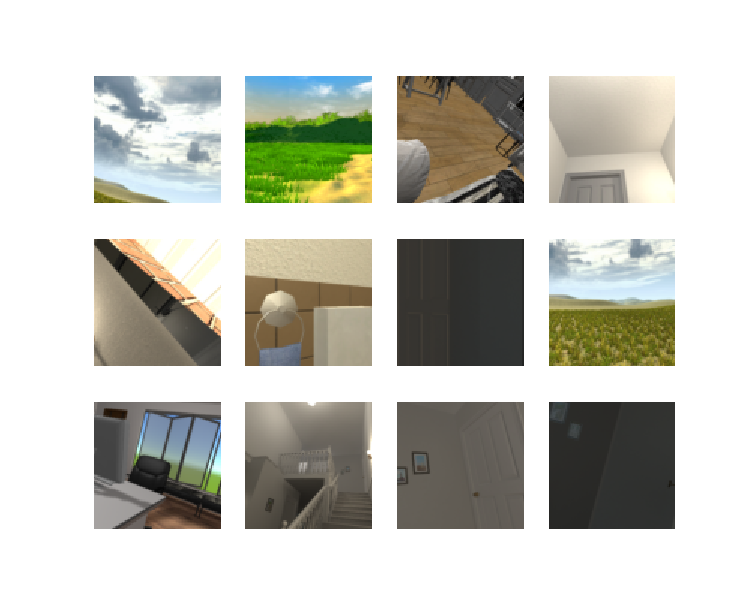
\includegraphics[scale = 0.55]{ProgressReport/eda-2.pdf}
    \caption{There are many synthesised images in this dataset, which could make the classification task more difficult.}
    \label{eda}
\end{figure}
After exploratory data analysis, we found the dataset is composed by real images captured by camera and images synthesized by computer \ref{eda}. Because real and synthesized images may not come from same feature space, which make the task more difficult than usual.

\begin{table}
\begin{center}
\textbf{Imbalanced Dataset Description}
\label{dataset}
\begin{tabular}{lcccc}
\hline Location & Classes & No. of Images \\
\hline
Interior & Bathroom & 704 \\
Exterior & Forest & 462 \\
Interior & Stairs & 703 \\
Exterior & Field & 1079 \\
Interior & Living room & 950 \\
Interior & Computer lab & 773 \\
\hline
\end{tabular}
\end{center}
\end{table}

%-------------------------------------------------------------------------
%%% Yufeng: Experiment Description includes at here.
\section{Related Works and Experiment Descriptions}
In this project, we are aimed to improve the validation accuracy of imbalanced scene dataset under limited computing resources. To get started, we first set a baseline experiment and then and 5 contrast experiments for comparison.
\subsection{Baseline:ResNet with Cross Entropy Loss}
ResNet \cite{resnet} was first proposed at 2015 for image classification. In this project, we use ResNet50 with cross entropy loss as our baseline. The batch size is 50, total epoch is 80 with learning rate 1e-4. 
\subsection{ResNet with AUC Maximization}
ROC curve plots the relationship between true positive rate and false positive rate. Higher slope of ROC curve indicates a higher ratio of true positive rate. AUC is defined as the area under ROC curve. Typically, a larger AUC value indicates the larger true positive ratio.According to the survey \cite{yang2022algorithmic}, the Multi-task AUROC loss function can be defined as:

\begin{align*}
&\min _{\mathbf{w} \in \mathbb{R}^d, \mathbf{a} \in \mathbb{R}^K, \mathbf{b} \in \mathbb{R}^K} \max _{\mathbf{s} \in \mathbb{R}^K} \\ 
&\sum_{k=1}^K \mathbb{E}_{\mathbf{x}_i \sim \mathcal{S}_{+}^k}\left[\left(h_{\mathbf{w}}\left(\mathbf{x}_i ; 
k\right)-a_k\right)^2\right] \\
&+\mathbb{E}_{\mathbf{x}_j \sim \mathcal{S}_{-}^k}\left[\left(h_{\mathbf{w}}\left(\mathbf{x}_j ; k\right)-b_k\right)^2\right] \\
&+s_k\left(\mathbb{E}_{\mathbf{x}_j \sim \mathcal{S}_{-}^k}\left[h_{\mathbf{w}}\left(\mathbf{x}_j ; k\right)\right]-\mathbb{E}_{\mathbf{x}_i \sim \mathcal{S}_{+}^k}\left[h_{\mathbf{w}}\left(\mathbf{x}_i ; k\right)\right] +c\right) \\
& -\ell^*\left(s_k\right)
\end{align*}
Where k represents the number of classes, $h_w(x;k)$ represents the predicted function, $\ell\left(\mathbf{w} ; \mathbf{x}, \mathbf{x}^{\prime}\right)=\ell\left(h_{\mathbf{w}}\left(\mathbf{x}^{\prime}\right)-h_{\mathbf{w}}(\mathbf{x})\right)$ denotes the surrogate loss function for a positive and negative pair, $l^*$ denotes its convex conjugate function, $c$ is the margin parameter.\\
Finding a stationary point with good performance for stochastic min-max optimization problem can be very difficult using traditional optimizer, in \cite{DBLP:journals/corr/abs-2012-03173}, they propose PESG method, which are a primal-dual method for solving stochastic min-max optimization problem with provable guarantees. In 2022, the optimization methods and loss function have been formalized in the library \cite{libauc2022}.In experiment, one-hot-encoding for label is used.The batch size is 50, total epoch is 80, margin parameter is set to be 0.95. The initial learning rate is 0.2 and the learning rate will adaptively decrease after 30 epochs.

\subsection{ Vision Transformer for Image Classification}
Since transformer and attention mechanism \cite{DBLP:journals/corr/VaswaniSPUJGKP17} was introduced , they have made great success in language processing. In the article \cite{DBLP:journals/corr/abs-2010-11929}, transformer structure was first introduced into vision tasks. Images are firstly cut into small patches. After that, send small patches into encoder with positional embedding connected with transformer and a multi-layer perceptron for classification. In our setting, we use pre-layer normalization transformer structure. Patch size for image processing is 32, the total number of patches are 49. The linear embedding is set to be 1024, the number of transformer blocks are 6 with the 8 heads. The dropout rate is 0.2.
For training, we set the learning rate to be $1e-4$, batch size is 50, the total epoch is 15.
\subsection{Zero-shot Learning using CLIP}
In this task, the technique of zero-shot learning with the CLIP\cite{DBLP:journals/corr/abs-1911-02685} is used. Instead of training the network by ourselves, Zero-shot learning is used for validation which enables model to recognize objects it has never seen. To utilize CLIP, we encode the text classification task through CLIP's text encoder to obtain text embedding, then encode the image using an encoder. By computing the similarity of embedding vectors of text and image, the index with highest similarity will be selected as the prediction output. The pretrained model parameters "ViT-B-32" is used for validation.

\subsection{Zero-shot Learning with ViT-GPT2 and FlanT5}
The flow chart \ref{FlanT5} described this experiment. Similarly as previous section, zero-shot classification is used in this part. Inspired by image to text technique introduced by \cite{abeywardana_2021}, we want to utilize ViT-GPT2 network structure to transform the image content into text descriptions. Then, send the text descriptions into FlanT5 model and specify the task as a classification task. Finally, compare the output text label with true text label and compute the validation accuracy.

\begin{figure}
    \centering
    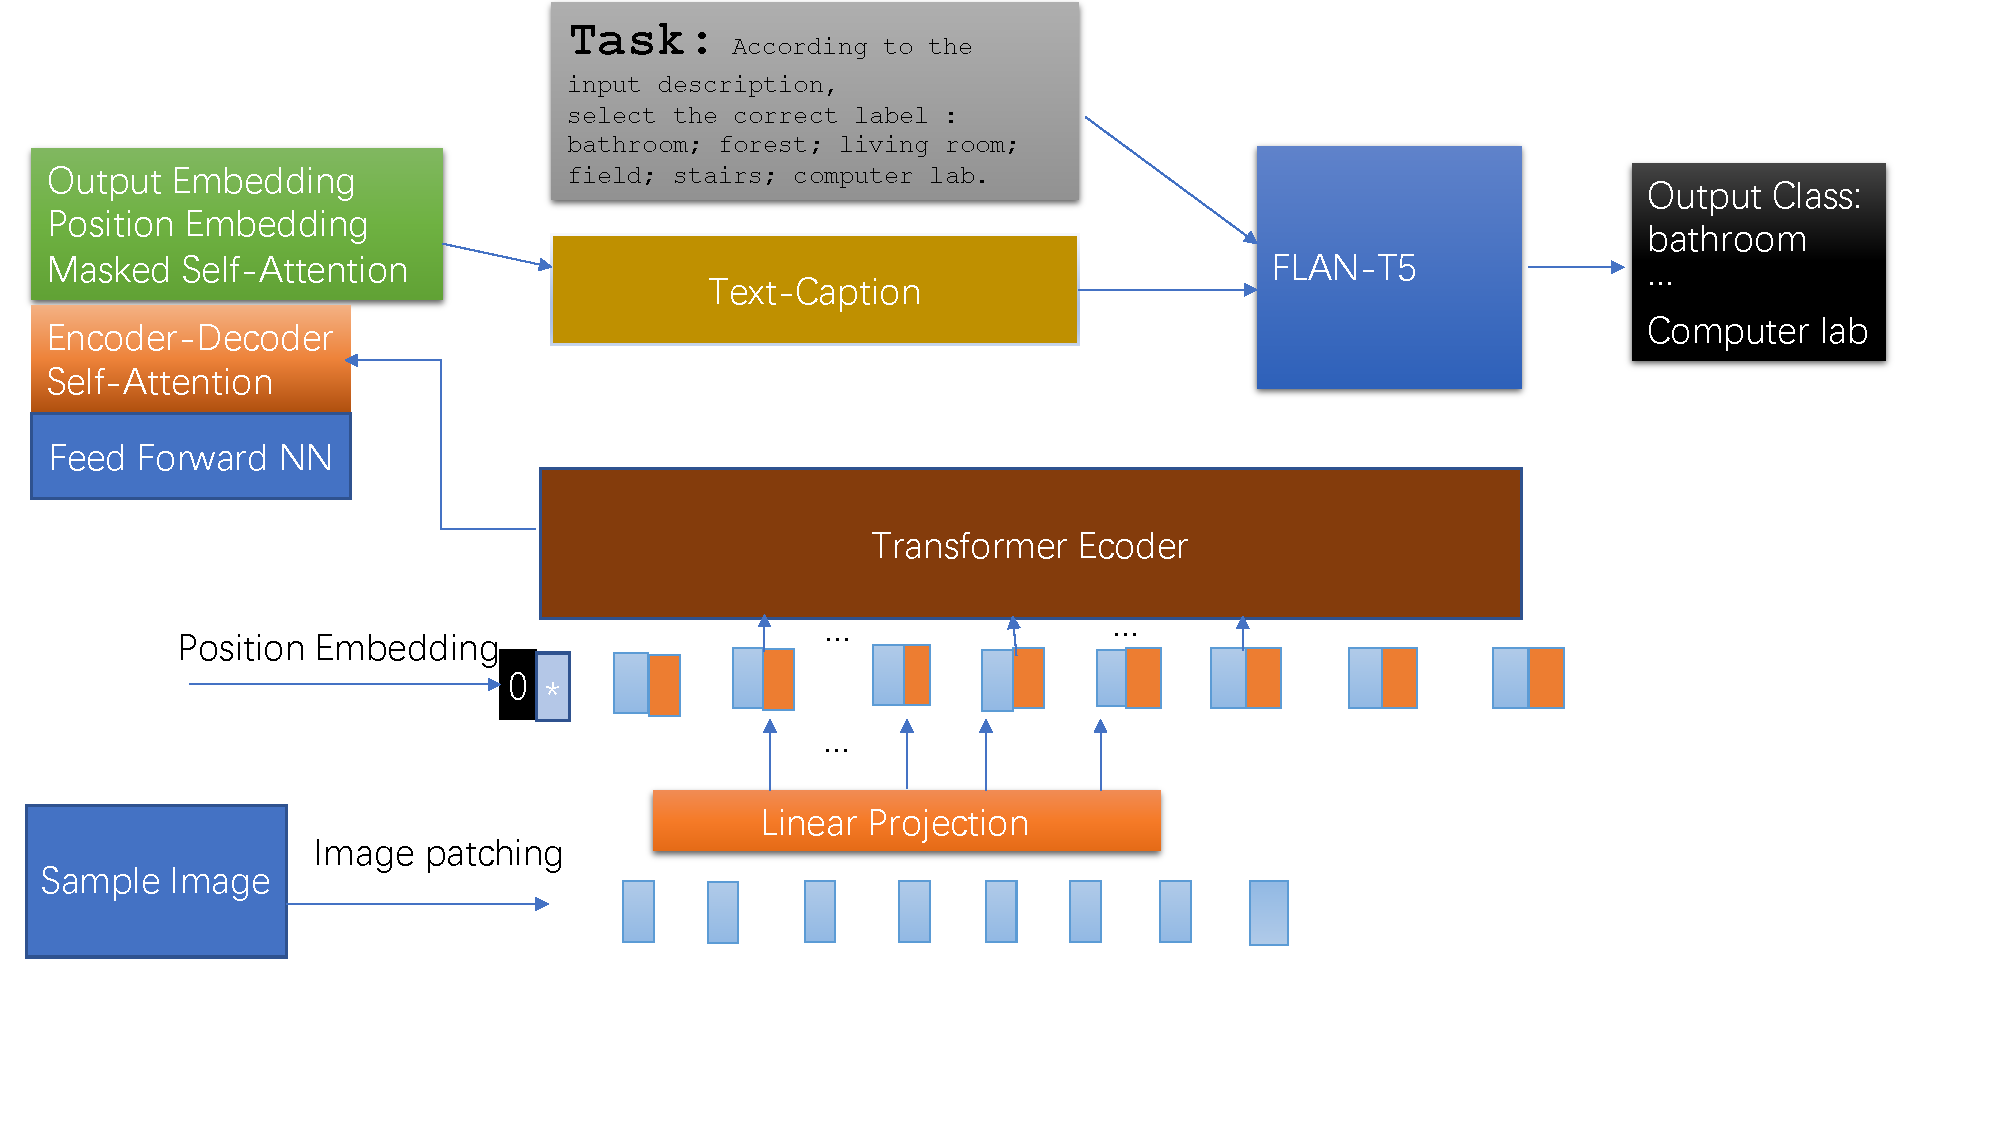
\includegraphics[scale = 0.25]{ProgressReport/Demo.pdf}
    \caption{Flow chart of ViT-GPT2+FlanT5}
    \label{FlanT5}
\end{figure}
\subsection{ Knowledge Transfer with fine Tuning}
According to the survey paper \cite{DBLP:journals/corr/abs-1911-02685},Transfer learning is a technique where pre-trained model is fine-tuned for a different but related task. When model is already trained on a large dataset with various categories, the model is expected to generalize its knowledge for different tasks and thus reduce the need for data labeling and large amount of computational resources.\\
In experiment, ResNet50 is used. The weight parameters initialized are obtained by training the ImageNet1k dataset, which contains approximately 1 million images, spanning 1,000 different categories. The tuning epochs are 30, learning rate is $1e-4$,batch size is 50. The reason for decreasing epochs number and learning rate is because we want to keep the wider knowledge of the initialization has and use it to adapt to our problems.
\begin{table*}[h]
\begin{center}
\resizebox{165mm}{!}{
\begin{tabular}{ l  l  c  c  c }
\toprule
\textbf{Method} & \textbf{Trained or Not} & \textbf{Number of Epochs} &\textbf{max train accuracy} & \textbf{max val accuracy}  \\
\midrule
ResNet50+CrossEntropy+Adam & $\checkmark$ & 80 & 69.1$\%$ & 79.3 $\%$ \\
ResNet50+AUROC(Multi-task)+PESG& $\checkmark$ & 80 & 83.5 $\%$ & 83.9 $\%$ \\
Vision Transformer+CrossEntropy+Adam & $\checkmark$ & 15 & 99.4 $\%$ & 99.7 $\%$\\
Zero-shot CLIP & $\times$ & NA & NA & 73.83 $\%$\\
Zero-shot ViT-GPT2+FlanT5 & $\times$ & NA & NA & \textbf{100}$\%$ \\
Transfer Learning (imagnet1k) & $\checkmark$ & 30 & \textbf{100}$\%$ & \textbf{100}$\%$ \\
\bottomrule
\end{tabular}}
\end{center}
\caption{Experiment Setting and Results for proposed models.}
\label{table:results}
\end{table*}

\section{Experimental Results}
The table \ref{table:results} shows our experiment setting and validation accuracy in details.
\subsection{Train ResNet with Cross Entropy and Adam}
According to figure\ref{basline exp} and result\ref{table:results}, the validation accuracy starts from 20$\%$ and grow slowly to 86$\%$. But this process is relatively slow. In the following parts, our aim is to improve the result within less epochs.

\begin{figure}[ht]
    \centering
    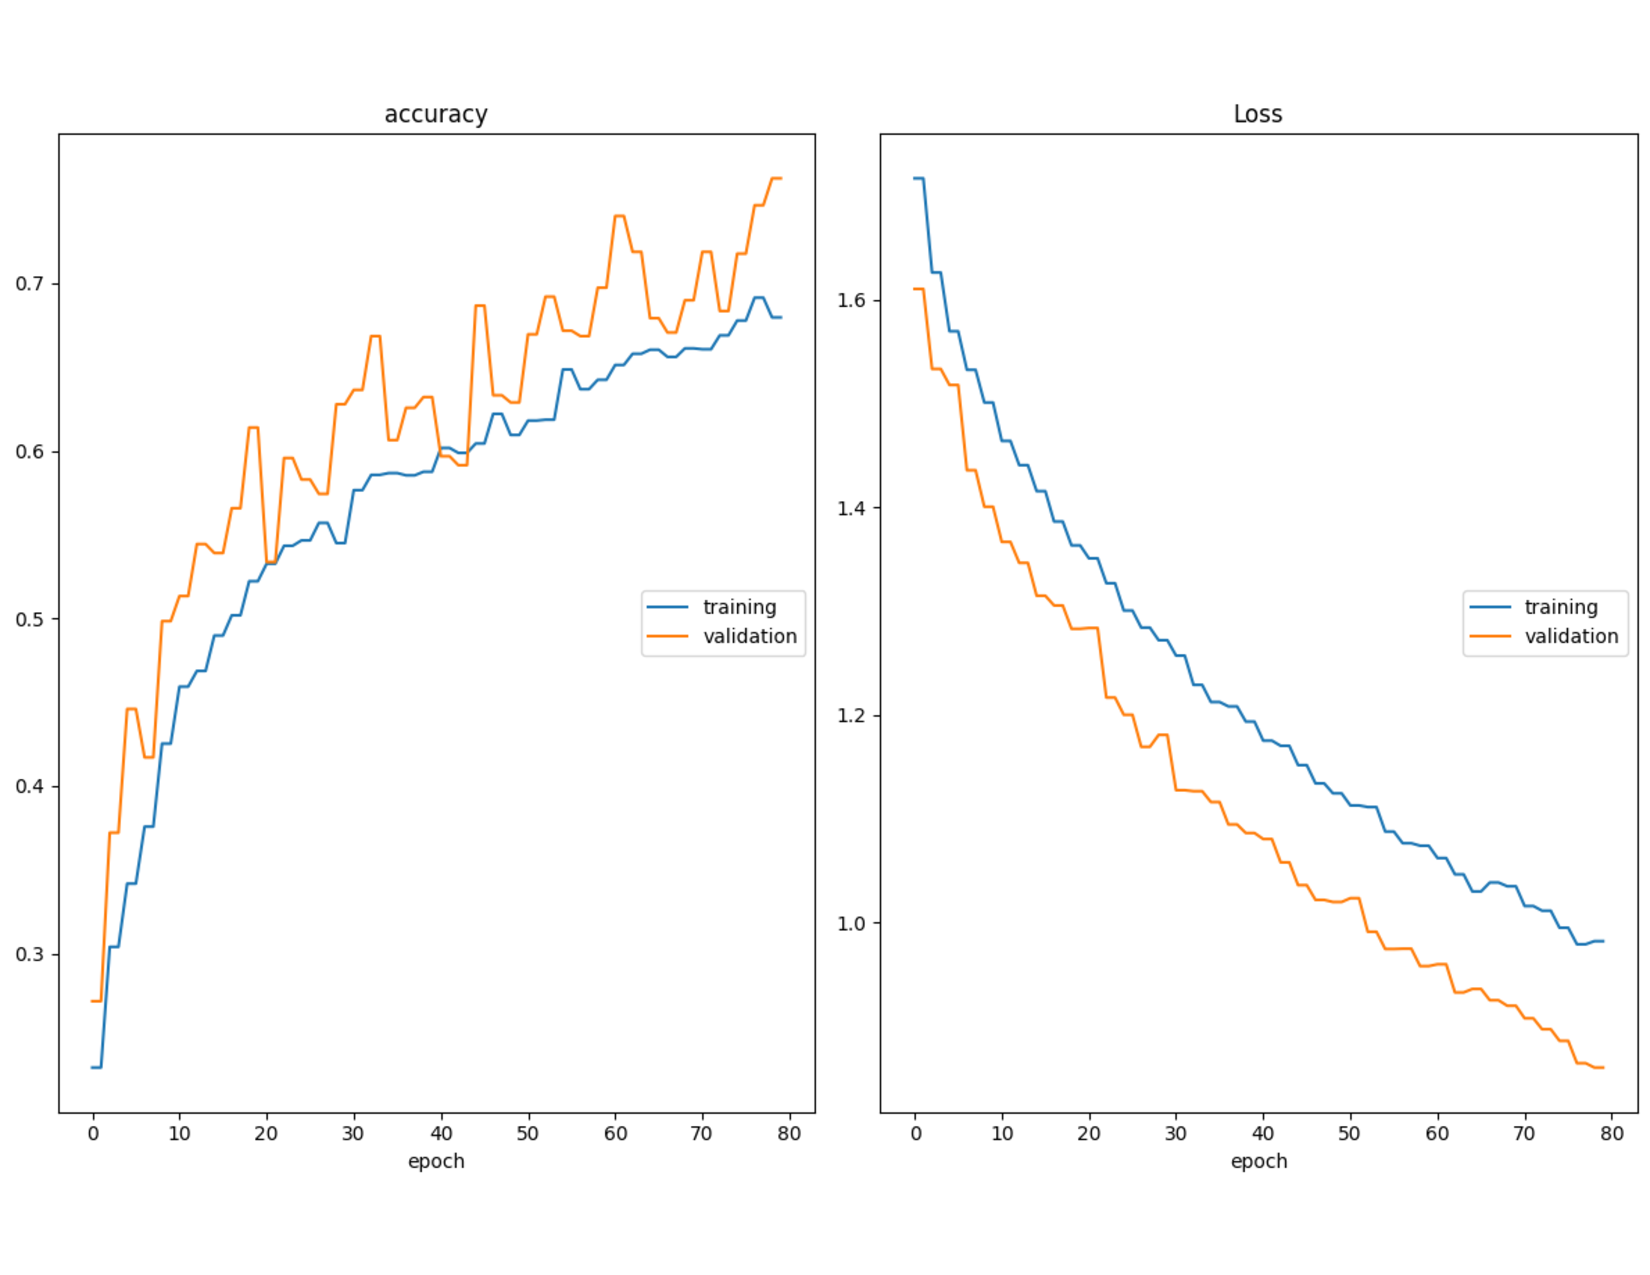
\includegraphics[scale = 0.3]{ProgressReport/CE_ResNet.pdf}
    \caption{ResNet50+CrossEntropy+Adam}
    \label{basline exp}
\end{figure}




\subsection{Train ResNet with AUROC loss and PESG}
According to result\ref{table:results}, although validation accuracy by training AUROC loss has achieved over 80$\%$ after 40 epochs, we found optimizing AUROC loss function is extremely tricky. From the loss graph \ref{AUC},the loss function will stay at certain level for a long time before updating. This is because of the problem formulation is a min-max stochastic optimization problem, which might have many non-degenerate saddle point. In order to efficiently escape from saddle point, sufficient large learning rate is required. we initialize the learning rate to 0.2 and enforce the learning rate to decrease adaptively after 30 epochs. \\
Besides, we found although the average AUC score has increasing trend. Check the AUC score for each class at last iteration: $\left [ 1.0, 1.0, 0.99,1.0,1.0,0.07 \right ]$. We found AUC score for computer lab is extremely low, which is not accepted. To conclude, AUC maximization still has several drawbacks on this imbalanced dataset and more advanced experiments are required.

\begin{figure}[ht]
    \centering
    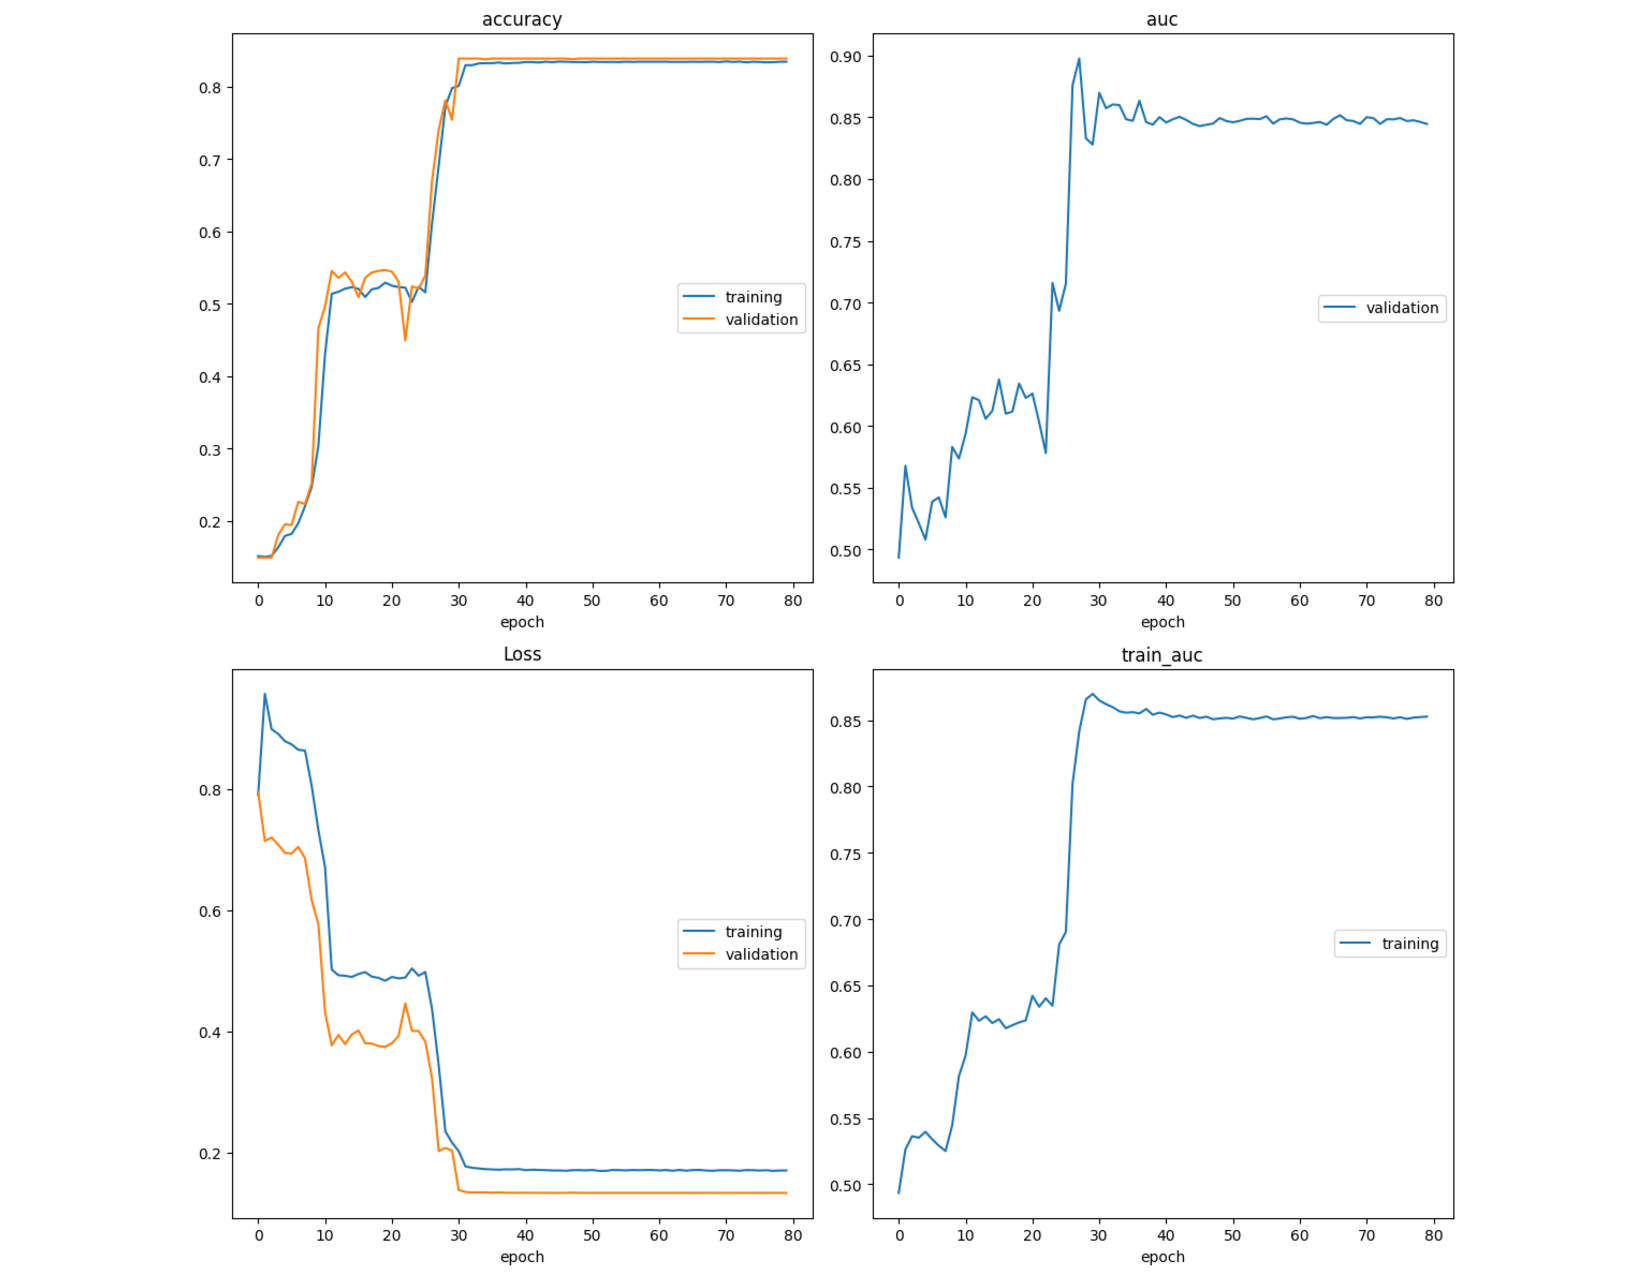
\includegraphics[scale = 0.33]{ProgressReport/AUC.pdf}
    \caption{ResNet50+AUROC+PESG}
    \label{AUC}
\end{figure}


\subsection{Train Vision Transformer with Cross Entropy and Adam} 
Firstly, we need to cut images into small patches. The visualization of patched images for different classes at figure\ref{image patch}. From here, we found patched images from different classes have obvious differences, which enables the network to classify the image class more easily.
According to result\ref{table:results} and figure\ref{Vision Trans}, the accuracy coincides with our explanation.  Within few epochs, the validation accuracy has exceeded 95$\%$.
\begin{figure}[ht]
    \centering
    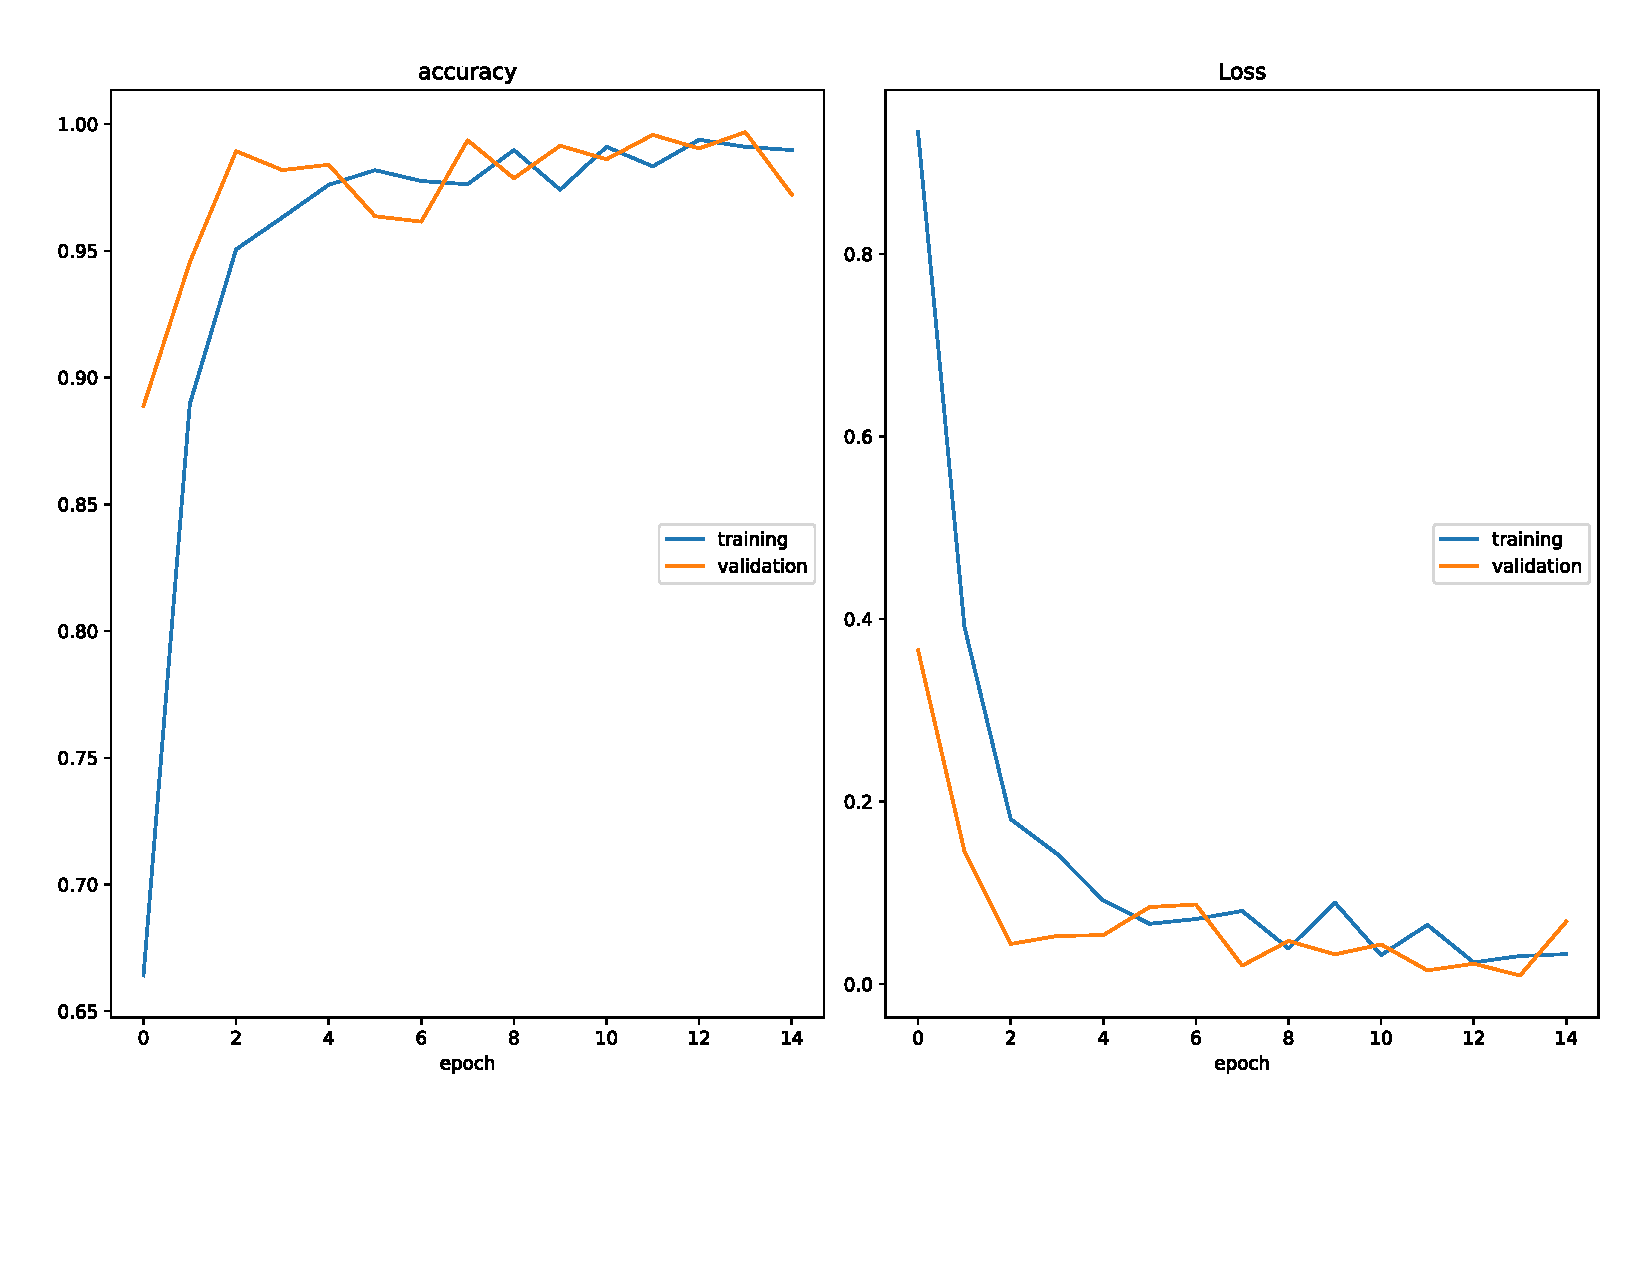
\includegraphics[scale = 0.3]{ProgressReport/ViT_2.pdf}
    \caption{Vison Transformer+Cross Entropy+Adam}
    \label{Vision Trans}
    
\end{figure}

\begin{figure}[h]
\centering

\includegraphics[width = 90mm,height = 30mm]{ProgressReport/image_patch-2.pdf}
\caption{Pattern for Patched Images}
\label{image patch}
\end{figure}
\subsection{Zero-shot Learning using CLIP}
According to the result \ref{table:results}, the validation result is only 73.83$\%$, which is lower than expectation. However, Recall the visualization of dataset \ref{dataset}, some images are too dark to classify. Thus, The possible reason behind this result might be the ill-conditioned image, which lacks semantic and text prompting information to classify them with correct labels. 
\subsection{Zero-shot Learning using ViT-GPT2+FlanT5}
To improve previous experiment, we replace image encoder by a well-trained image-to-text network, which is aimed to caption the information images include. The following table \ref{text output} shows some sample output of ViT-GPT2.After obtaining the text output, we use these descriptions as inputs to FlanT5. Results \ref{table:results} showed that it 100$\%$ match the text with correct label.\\
This is not surprising if we think about the casualty between text input and text label, which is stronger than images with respect to label. The intervention probability used in casual inference is defined as $P(y \mid do(x), z)$, which captures the probability of y happens if we do event x. Obviously, by observing the text in table, it is much easier to have a correct guess by looking at images \ref{dataset}, which means $P(y \mid do(x), z)$ is higher if event x is the text input.
\begin{table}[h]
\begin{center}
\textbf{Sample Generated Text Output}
\label{text output}
\resizebox{\columnwidth}{!}{
\begin{tabular}{lcccc}
\hline Sample Output \\
\hline
"a white toilet sitting next to a bath tub" (bathroom)\\
"tree in the middle of a forest" (forset)\\
"black and white photo of a stairway with stairs" (stairs)\\
"a field with a bunch of green grass" (field)\\
"a living room filled with furniture and a window" (livingroom)\\
 "two computer monitors sitting side by side on a desk" (computer lab) \\
\hline
\caption{Sample Output Generated by ViT-GPT2}
\end{tabular}}
\end{center}
\end{table}
\subsection{Transfer Learning for image classification }
According to figure\ref{Transfer} and result\ref{table:results}, the starting training and validation accuracy has exceeded 90$\%$. This is because the weight learned by training ImageNet1k dataset has strong generalization capability. After several epochs' tuning, the validation and training accuracy is vibrated a little bit and even decrease, this is because of the training process break the knowledge learned from ImageNet1k, where the generalization capability is decreased. Thus, a small learning rate and epoch number are important for this experiment.
\begin{figure}[t!]
    \centering
    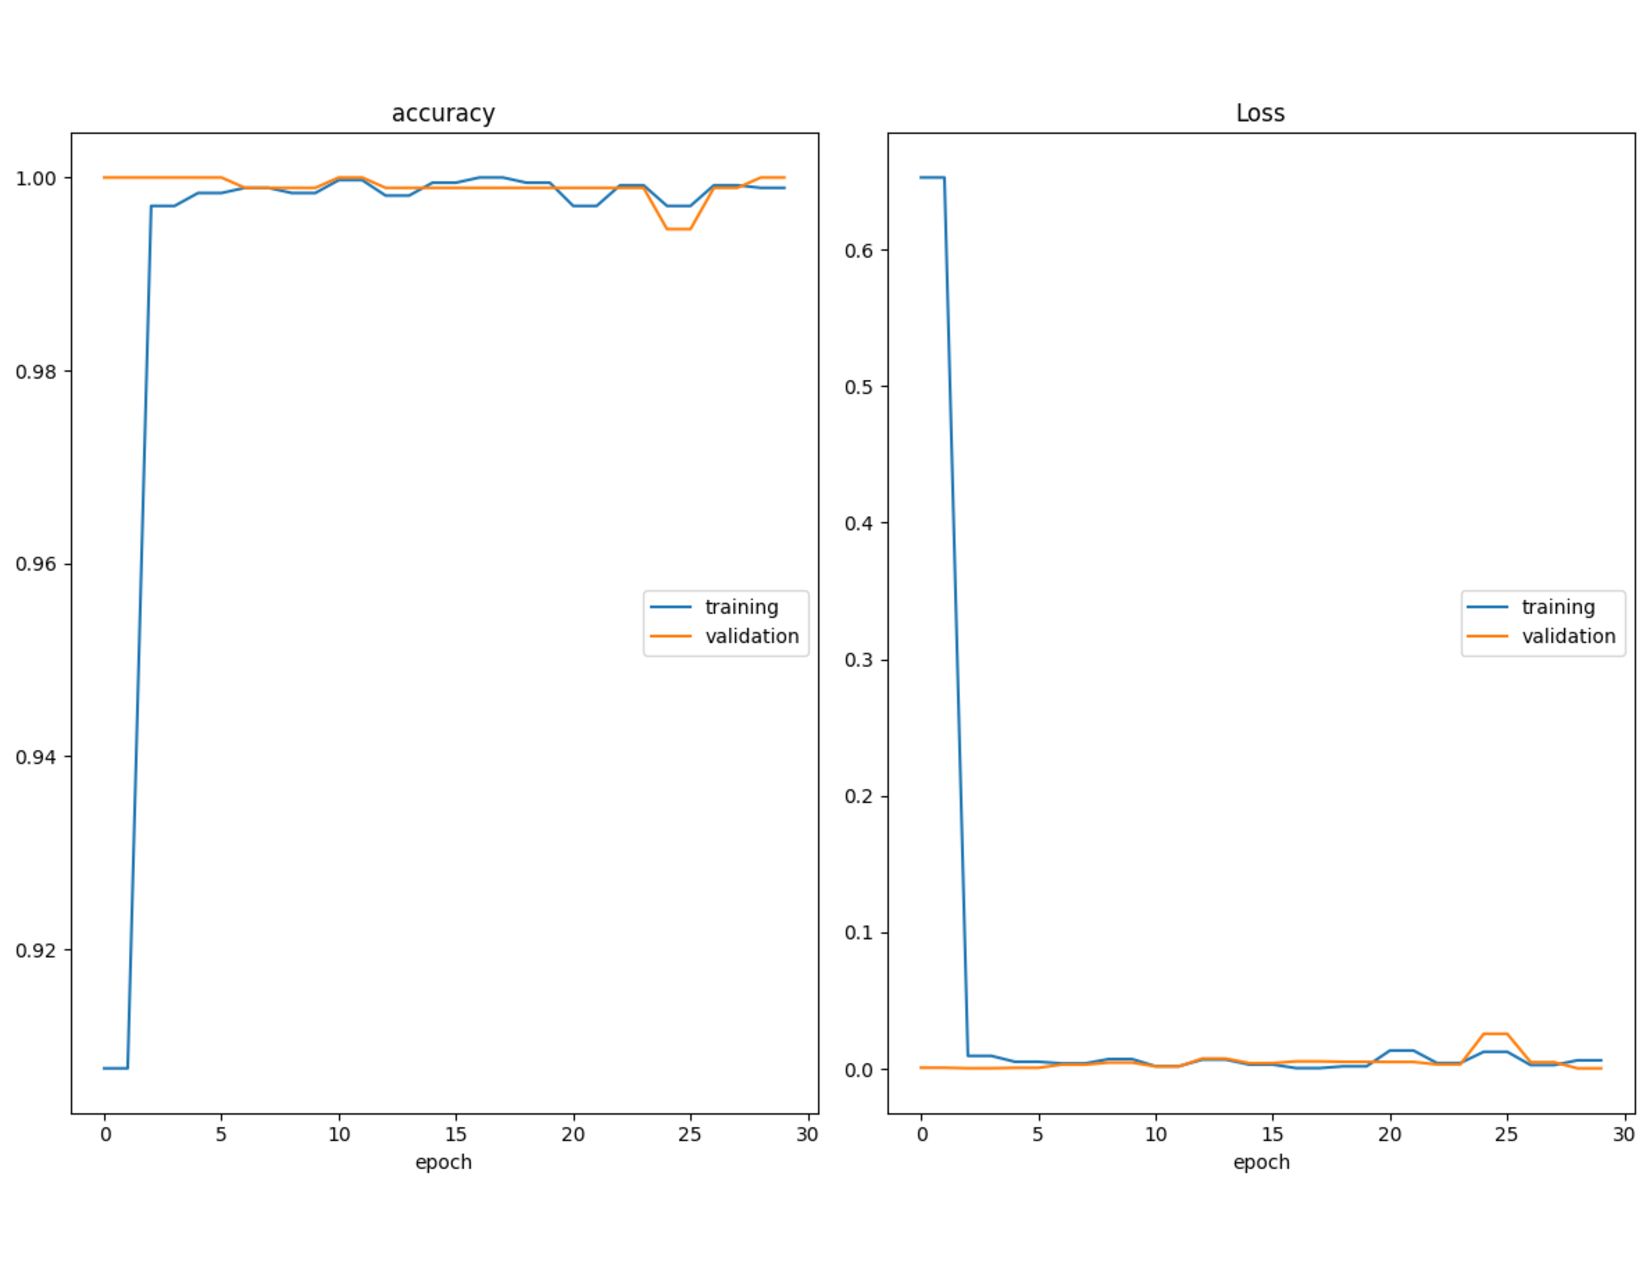
\includegraphics[scale= 0.3]{ProgressReport/Transfer_Learning.pdf}
    \caption{Transfer Learning (from ImageNet1k)+Cross Entropy+Adam}
    \label{Transfer}
\end{figure}
\section{Conclusion and Future Work}
In this work, an imbalanced dataset mixing real images and synthetic images is used to represent an "unfair" dataset. Our experiment is aimed to modify network structure and improve learning paradigm to make the overall classification accuracy as high as possible.Experimental results indicate AUC maximization can save computing resources but is hard to train. Transformer network structure can improve the overall classification a lot with fewer epochs. Furthermore, it is showed that utilizing a powerful pre-trained model and the information from multi-media can significantly improve the classification accuracy and save our computing resources.This enables us to see the generalization capability of model parameterized by the model trained on high-quality large-scale data.\\
However, it is always worthwhile to think about how to improve the model validation accuracy under unfair distribution where some classes of images are lacked. This work gives us two streams to resolve this issue. The first is to improve the network structure. For example vision transformer is verified with better performance in this project. In future, people can also try GAN\cite{goodfellow2014generative}, condition GAN\cite{mirza2014conditional} or utilizing the concept of ensemble learning, which is proved to be effective for model robustness by J. Jia et al\cite{DBLP:journals/corr/abs-2008-04495} . Another stream is utilizing the weight parameters learned from a large dataset with good quality, for example, the concept of meta learning \cite{DBLP:journals/corr/FinnAL17} and transfer learning \cite{DBLP:journals/corr/abs-1911-02685} make the network parameter adapt to more complex tasks and ill-conditioned dataset. Hopefully, this work will give followers the awareness of fair issues in modern machine learning and inspire future works to improve model performance as well as AI ethics.





%%%%% DO NOT delete here, used for reference
{\small
\bibliographystyle{ieee}
\bibliography{egbib}
}

\end{document}
